\section{Experiments}
\label{sec:exps}
\subsection{Datasets}
To validate our methods, we evaluate on the publicly available dataset used in \cite{lejeune18}.
This consists in a variety of video and volumes of different modalities with 2D annotation points for different object types.
It includes:
\begin{itemize}
\item \textbf{Brain:} \(4\) 3D T2-weighted MRI scans chosen at random from the publicly available BRATS challenge dataset \cite{menze15}, where tumors are object of interest.
\item \textbf{Tweezer:} \(4\) sequences from the training set of the publicly dataset MICCAI Endoscopic Vision challenge: Robotic Instruments segmentation \cite{endochal}. The piecewise-rigid surgical instrument must be segmented.
\item \textbf{Slitlamp:} \(4\) slit-lamp video recordings of human retinas, where the optic disk is to be segmented.
\item \textbf{Cochlea:} \(4\) volumes of 3D CT scans of the inner ear, where the cochlea must be annotated. This object is the most challenging object to segment due to its complicated geometry.
\end{itemize}

\subsection{Proposed methods and baselines}
\label{sec:orge9e46ac}
\subsubsection{Baselines}
\label{sec:orgb4303b5}

We now evaluate the segmentation performance of the proposed foreground models with the following baselines.
\begin{itemize}
\item \ksp: Multi-object tracking method described in \cite{lejeune18}.
The foreground model is a bagging of decision trees similar to Random Forest.
\item \textbf{EEL}: An expected exponential loss to learn robust classifiers in a PU learning setting \cite{lejeune17}.
\item \textbf{Gaze2Segment}: A combination of saliency detection and graphcut \cite{khosravan16}.
\item \textbf{DL-prior}: Point location supervision is used to train a CNN with strong object priors \cite{bearman16}.
\end{itemize}

\subsubsection{Proposed}
\label{sec:org83c59ba}
\begin{itemize}
\item \puss: Non-negative positive-unlabeled (nnPU) with self-supervised class-prior estimation, as in Sec. \ref{sec:nnpu} and \ref{sec:pi_estim}.
\item \kspss: Combines the \puss method and the multi-object tracking refinement step of Sec. \ref{sec:tracking}.
\item \ksptrue: Same as above, except that the foreground model is the proposed CNN trained as in Alg. \ref{alg:sgdnnpu} using the groundtruth class-priors.
\item \kspconst: Same as above except we train Alg. \ref{alg:sgdnnpu} taking as prior a sequence-wise constant value given by the mean groundtruth prior over all frames.
\end{itemize}
For both \ksptrue{} and \kspconst{}, we train the foreground prediction model for $150$ epochs as in Alg. \ref{alg:sgdnnpu}. The learning rate is set to $10^{-4}$ and reduced to $10^{-5}$ after $50$ epochs.

\subsection{Segmentation performance}

We evaluate quantitatively the proposed methods (\puss{} and \kspss{}) to the baselines.
We set the initial upper-bound using the groundtruth annotations.
In particular, we compute for all frames the frequencies of positives $\pi^{i}$ and set $\hat \pi_{0}=1.4 \cdot \max_{i}{\pi^{i}}$.
As performance criteria, we use the F1 score, averaged on all $4$ sequences of a given type.
Quantitative results are shown in Tab. \ref{tab:results}.
Qualitative results are shown in Fig. \ref{fig:prevs}.

The \kspss{} method brings substantial improvement on the best baseline (\ksp{}) on all image modalities.
In particular, we report improvements in F1 scores of $18\%$ on Tweezer, $13\%$ on Cochlea, $9\%$ on Slitlamp, and $8\%$ on Brain.
Also, comparing \puss{} with \kspss{}, we quantify the added value of the proposed tracking module.
We report an improvement in average F1 score of $4\%$ on Tweezer, $41\%$ on Cochlea, $7\%$ on Slitlamp, and $6\%$ on Brain.

\begin{table*}[t]
\centering
\caption{
    Quantitative results on all datasets. We report the F1 scores and standard deviations.
    }
\label{tab:results}
\begin{tabular}{llp{1.8cm}p{1.8cm}p{1.8cm}p{1.8cm}p{1.8cm}}
\toprule
Types &               Tweezer &               Cochlea &              Slitlamp &                Brain \\
Methods         &                       &                       &                       &                      \\
\midrule
KSPTrack/nnPUss &  $\bm{0.91} \pm 0.03$ &  $\bm{0.75} \pm 0.05$ &  $\bm{0.84} \pm 0.05$ &  $\bm{0.8} \pm 0.09$ \\
nnPUss          &       $0.87 \pm 0.02$ &        $0.53 \pm 0.1$ &        $0.78 \pm 0.1$ &      $0.75 \pm 0.13$ \\
\hdashline
KSPTrack        &       $0.77 \pm 0.08$ &       $0.66 \pm 0.02$ &       $0.77 \pm 0.08$ &      $0.74 \pm 0.08$ \\
EEL             &        $0.6 \pm 0.16$ &       $0.12 \pm 0.05$ &       $0.59 \pm 0.08$ &      $0.52 \pm 0.14$ \\
Gaze2Segment    &        $0.18 \pm 0.0$ &       $0.07 \pm 0.02$ &        $0.02 \pm 0.0$ &      $0.07 \pm 0.02$ \\
DL-prior        &       $0.72 \pm 0.06$ &        $0.3 \pm 0.04$ &       $0.51 \pm 0.11$ &      $0.56 \pm 0.08$ \\
\bottomrule
\end{tabular}
\end{table*}


\begin{figure*}[t]
\caption{Qualitative results for each type. From left to right: Original image with groundtruth highlighted in red and 2D location in green, output of foreground prediction model (nnPUss), thresholded output of the latter, and segmentation using the full pipeline (KSPTrack/nnPUss).}
\centering
    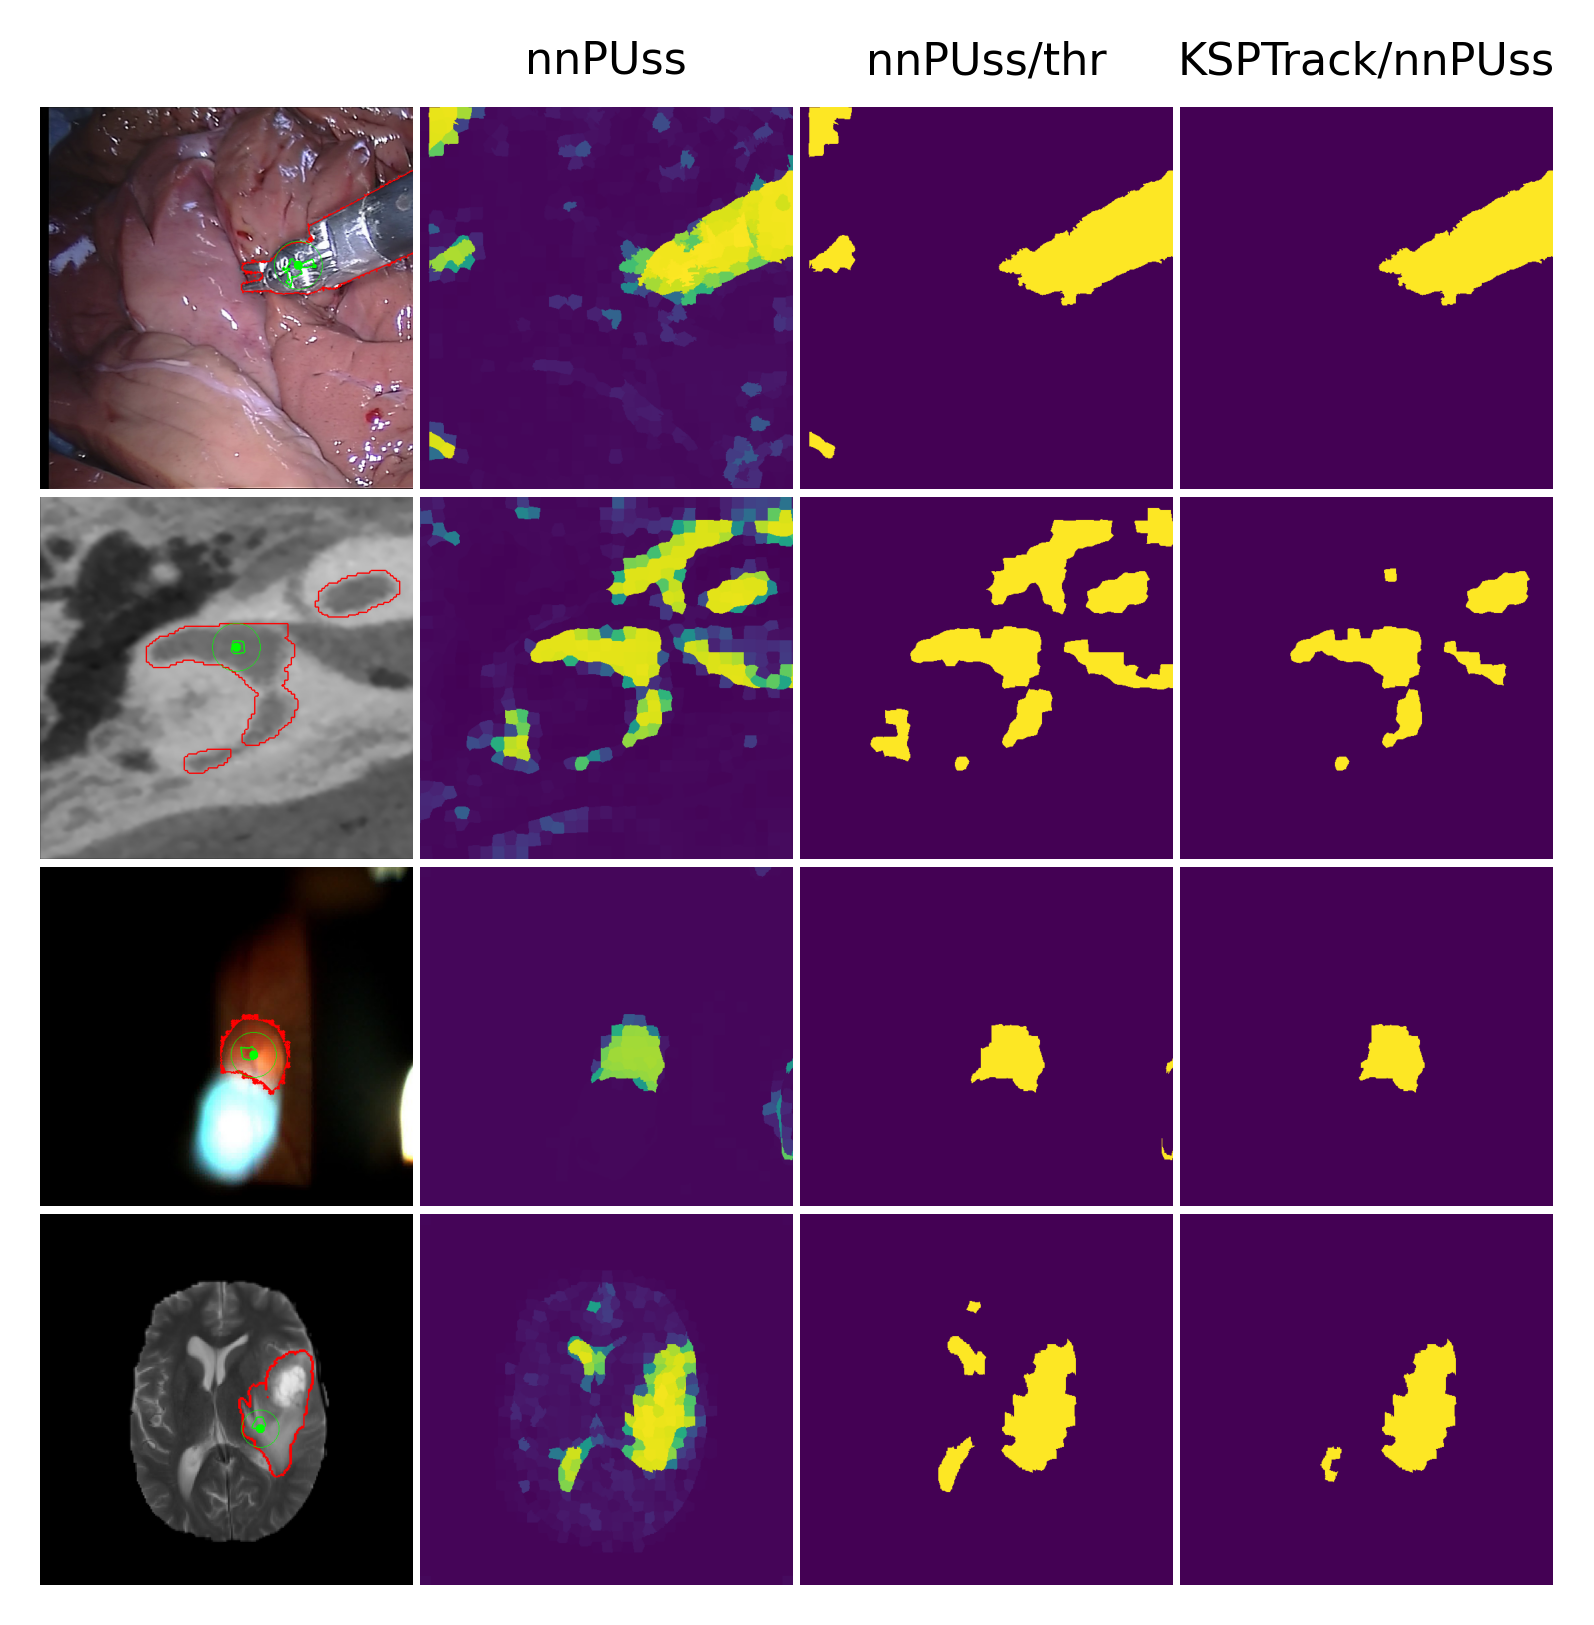
\includegraphics[width=.6\textwidth]{pics/prevs.png}
\label{fig:prevs}
\end{figure*}

\subsection{Analysis of Convergence}
\label{sec:convergence}

Fig. \ref{fig:converge} shows for each type of sequence the convergence of our class-prior estimation procedure (Sec. \ref{sec:pi_estim}).
All sequences are trained using $\hat\pi_{0}= 1.4 \cdot \max_i{\pi^i}$.

As we aim at estimating the true class-prior, we plot on the top panels the Mean Absolute Error (MAE) between the estimated priors and the true priors.
The proposed stopping condition, which leverages the variance of pseudo-negatives, is plotted in the bottom panel.

We observe that the proposed stopping condition triggers reasonably close to the optima in most cases.


\begin{figure*}[t]
\caption{For each type, we show: (top) Mean Absolute Error (MAE) between the predicted positive frequency of the classifier and the true prior (bottom) Variance of the pseudo-negatives, with threshold in dashed-red, and the minimum number of epochs in dashed-green.}
\centering
\begin{tabular}{@{}cc@{}}
    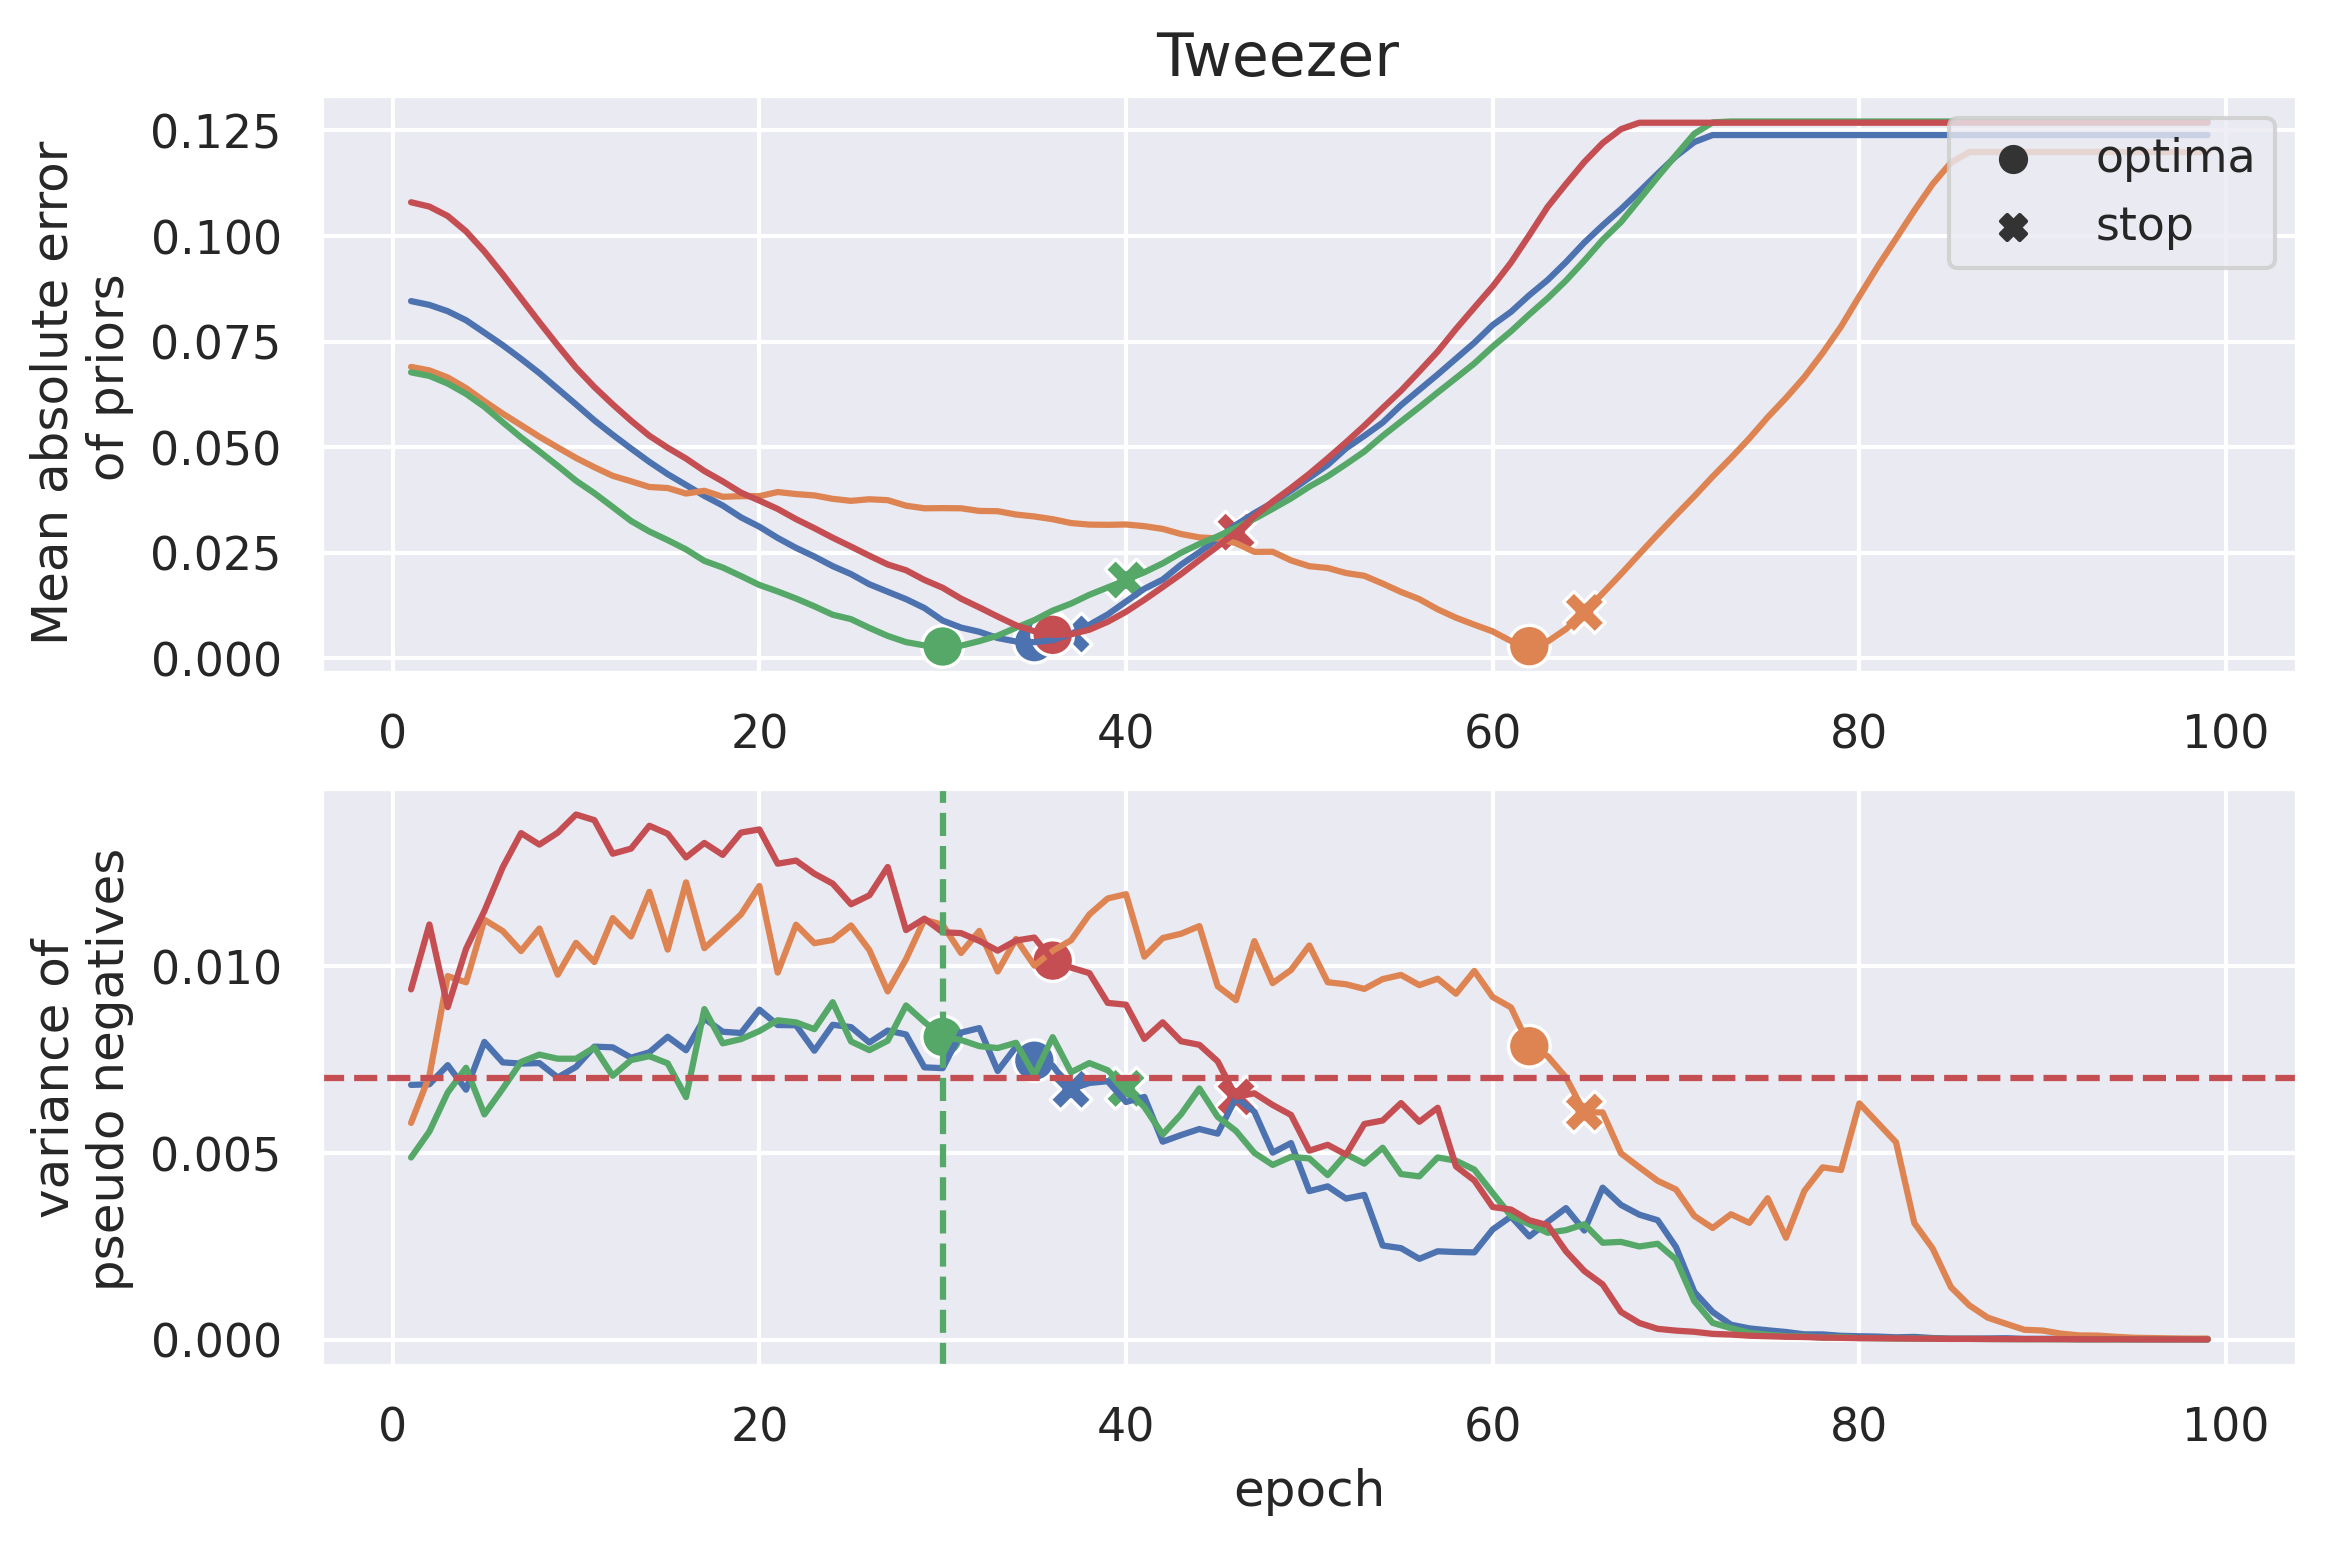
\includegraphics[width=.5\textwidth]{pics/tweezer_priors.png} &
    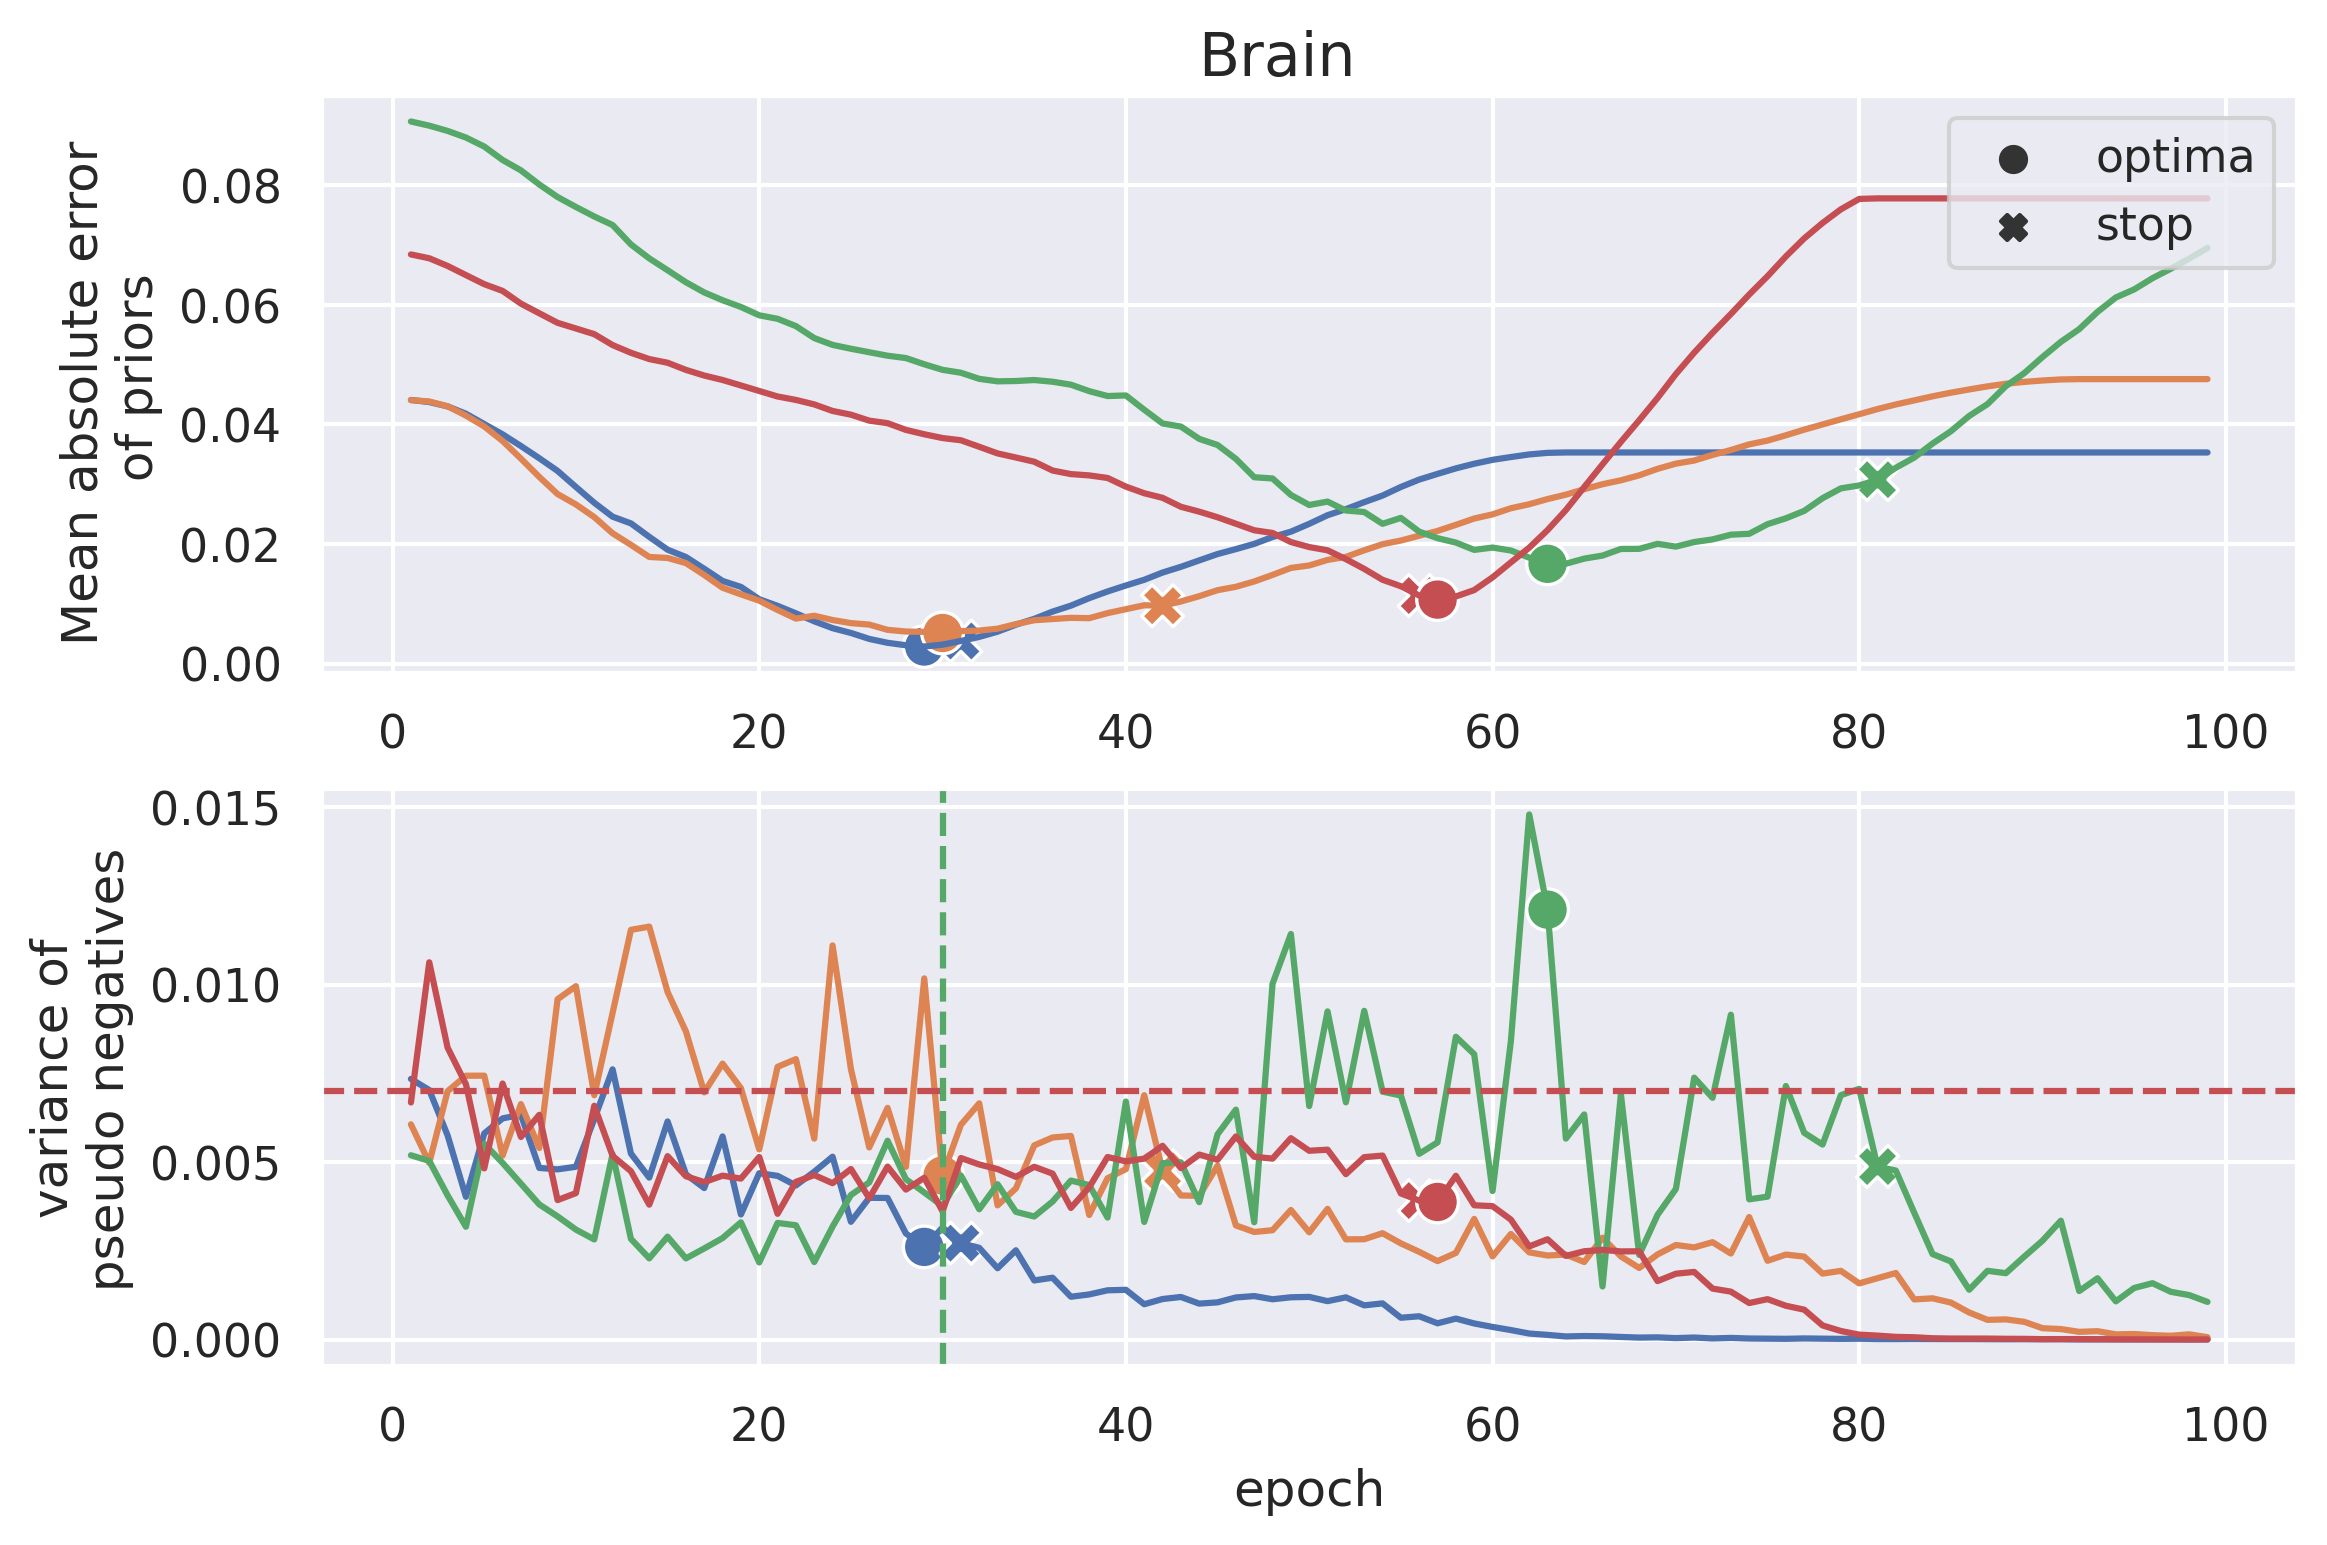
\includegraphics[width=.5\textwidth]{pics/brain_priors.png} \\
    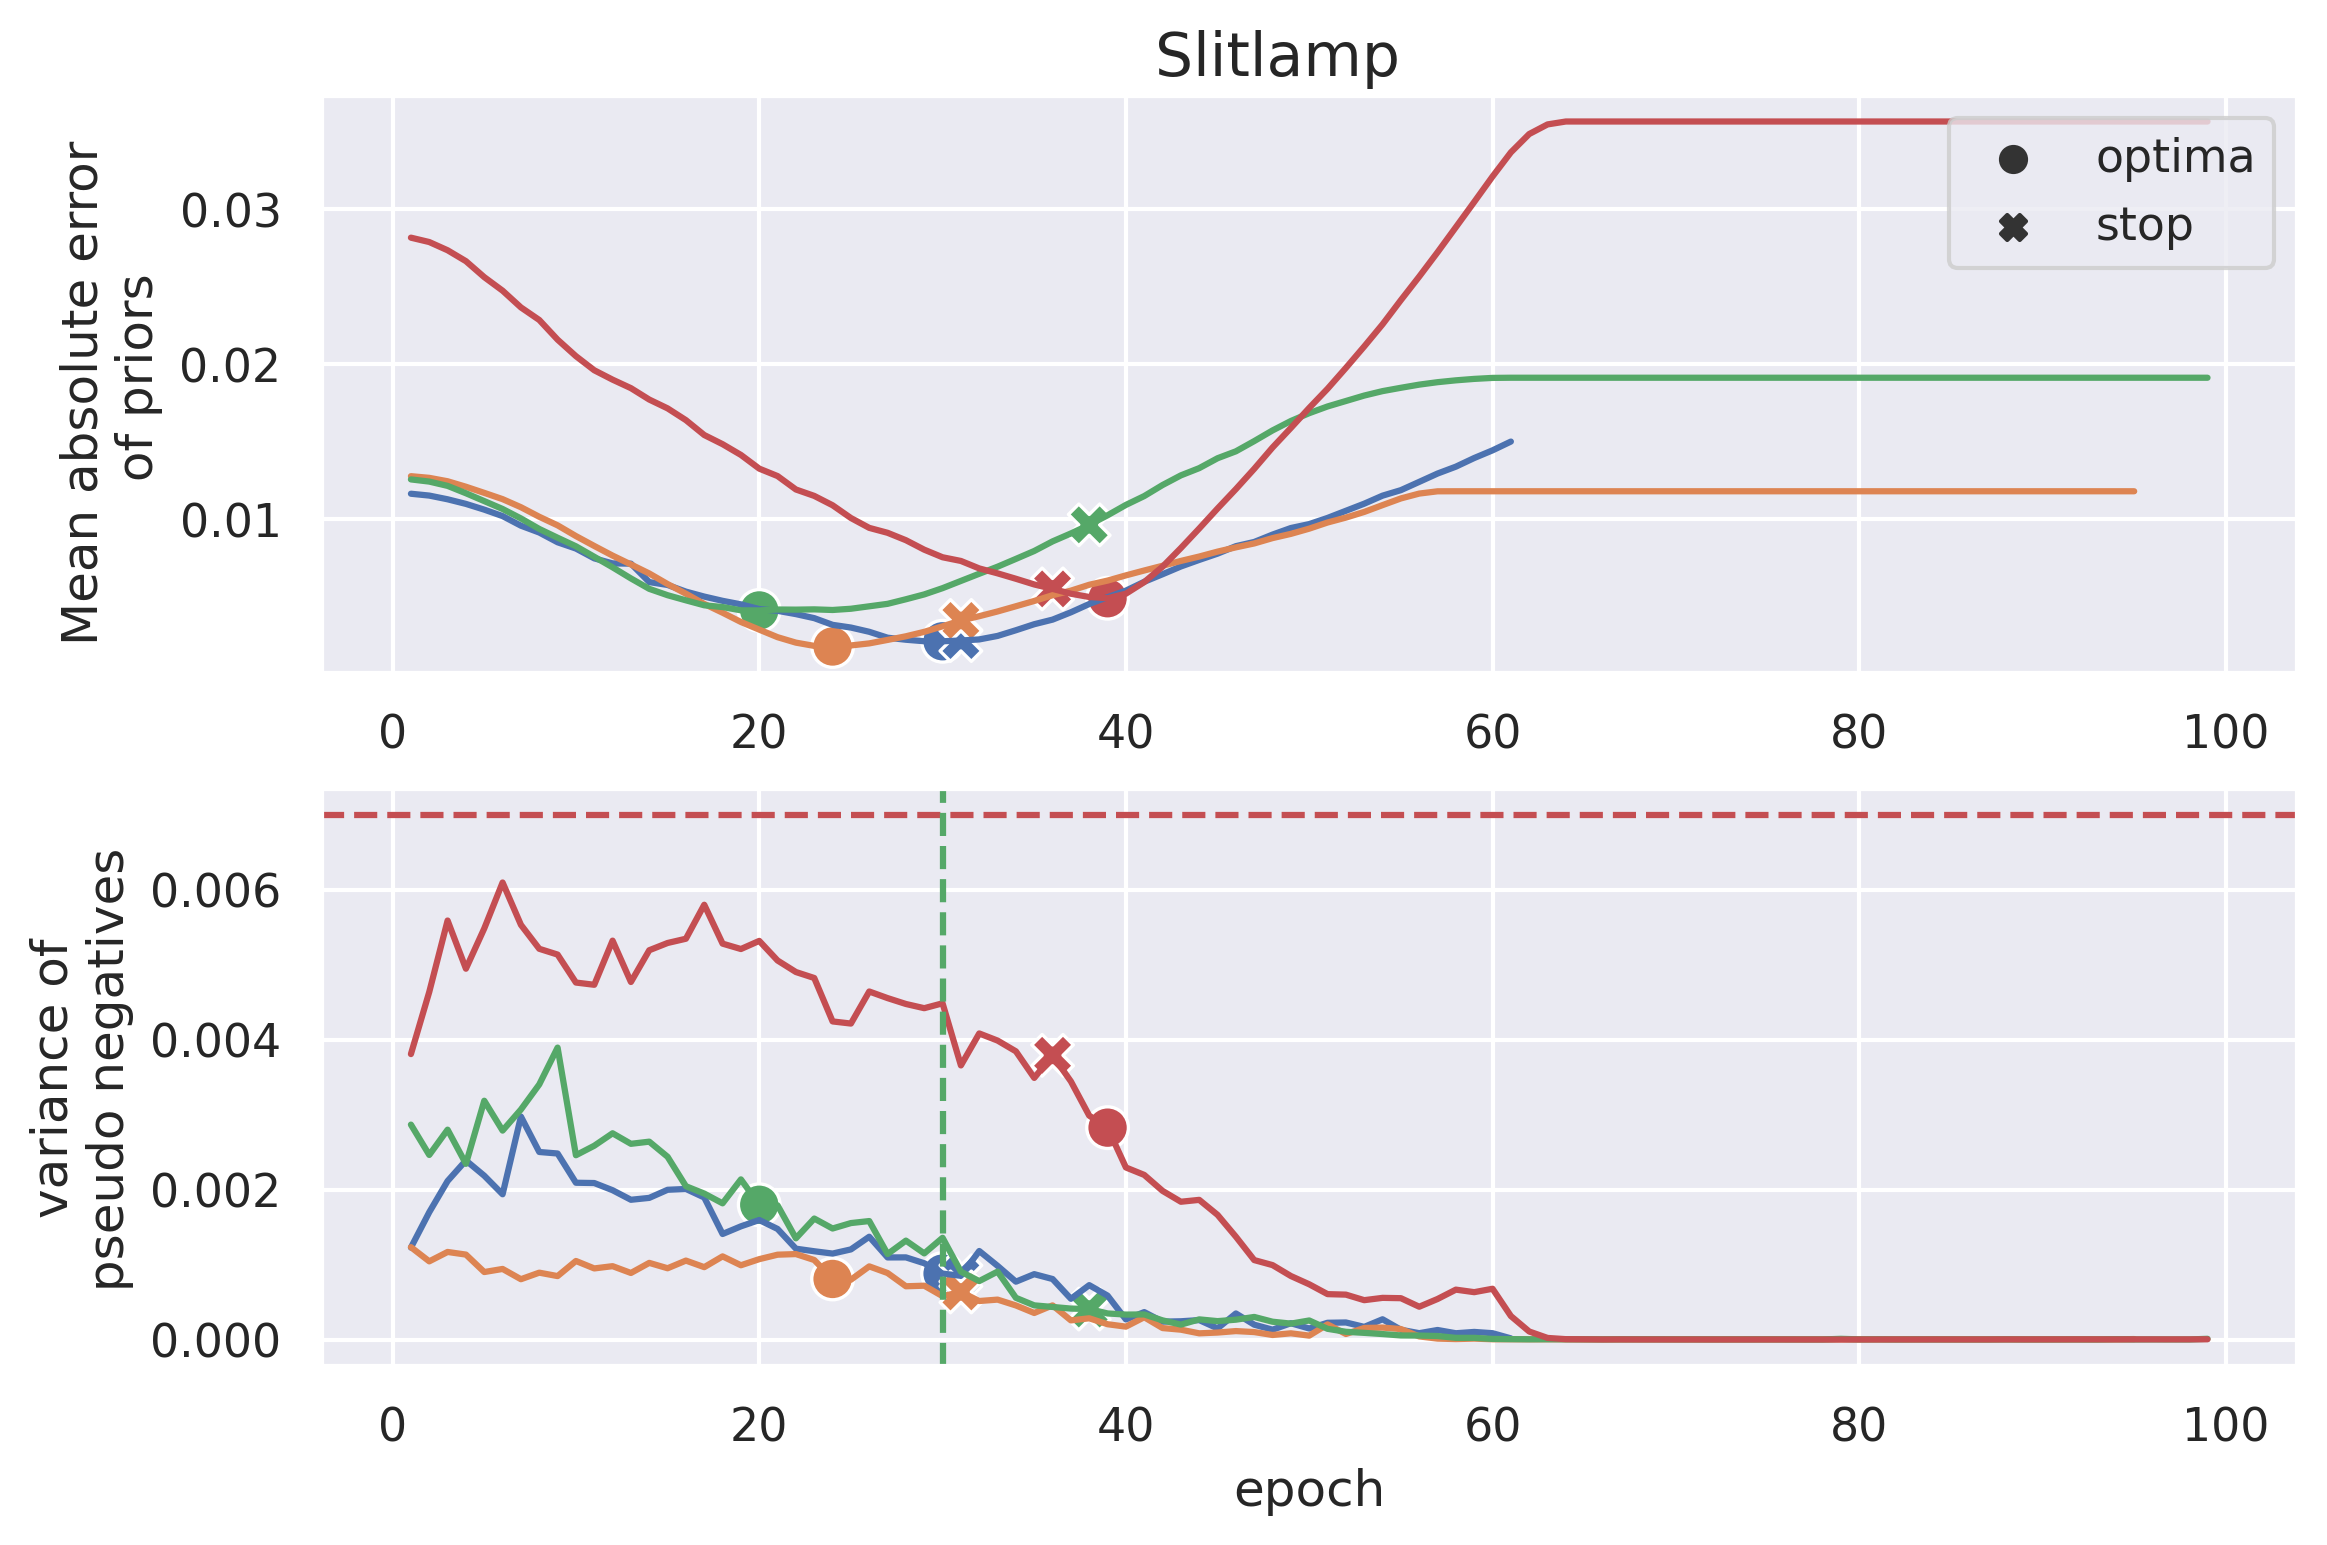
\includegraphics[width=.5\textwidth]{pics/slitlamp_priors.png} &
    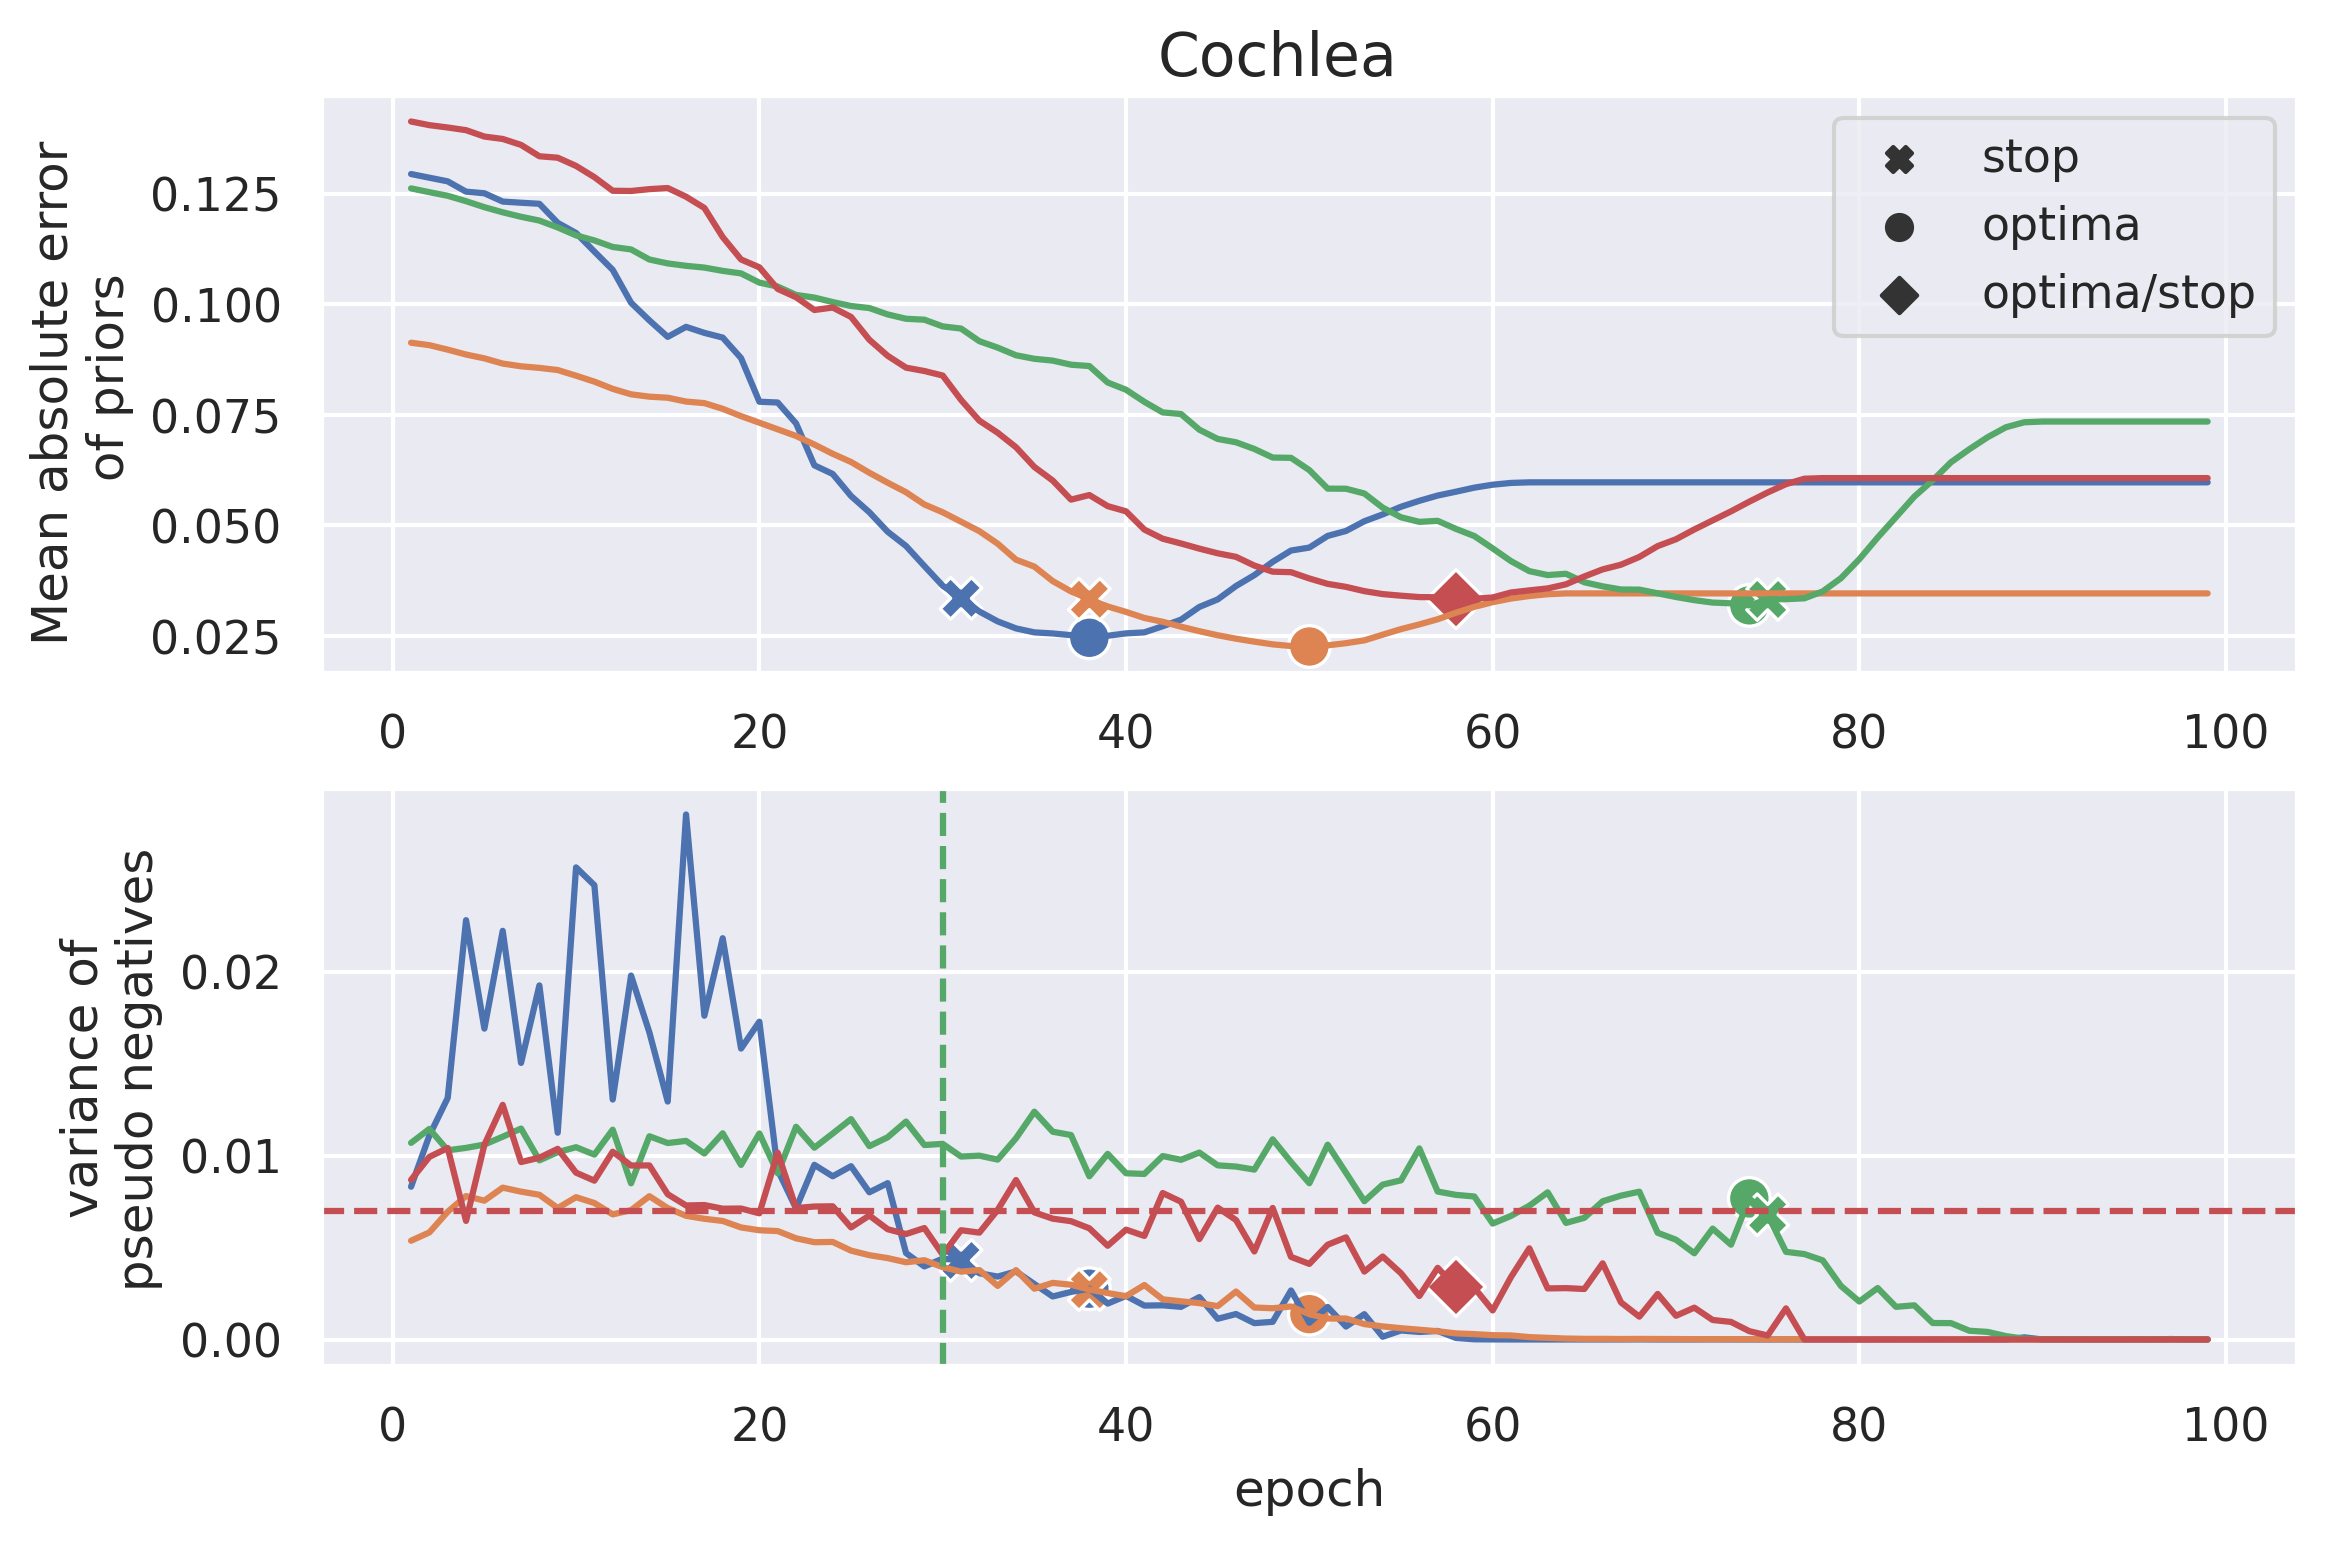
\includegraphics[width=.5\textwidth]{pics/cochlea_priors.png} \\
\end{tabular}
\label{fig:converge}
\end{figure*}

\subsection{Robustness w.r.t. upper-bound and relevance of frame-wise estimation}
\label{sec:org1ddd2fc}
We wish to assess how our self-supervised prior estimation method performs in a real-world scenario, where the provided upper-bound $\hat \pi_{0}$ is misspecified.
We therefore apply the proposed method \kspss{} using $\hat \pi_{0}=\eta \cdot \max_{i}\pi^{i}$, with $\eta \in \{1.2, 1.4, 1.6, 1.8\}$.
Also, in order to assess the relevance of the self-supervised estimation of priors, we perform segmentation using method \kspconst{} with $\eta \in \{0.8, 1.0, 1.2, 1.4\}$.
As reference, we further segment using the frame-wise true priors, as in method \ksptrue{}.
We report the F1 score, precision and recall in Tab. \ref{tab:results_eta}.

First, we observe that our self-supervised estimation of priors is relatively robust to variations of $\hat \pi_{0}$.
In particular, Tweezer shows variations in F1 scores of max. $1\%$ while $\eta$ varies over range $[1.2, 1.6]$.
Cochlea, varies by $4\%$ over range $[1.2; 1.6]$.
Slitlamp varies by $5\%$ over range $[1.4, 1.8]$.
Last, Brain varies by $4\%$ over range $[1.2, 1.6]$.

These variations are in general more important when using the simpler \kspconst.
In particular, Tweezer varies by $1\%$ over range $[0.8, 1.2]$,
Cochlea varies by $5\%$ over range $[1., 1.4]$,
Slitlamp varies by $15\%$ over range $[0.8, 1.2]$,
and Brain varies by $8\%$ over range $[0.8, 1.2]$.

The relevance of the frame-wise prior estimation is assessed by comparing, for each type, the maximum F1 scores reached by \kspss{} and \kspconst{} for all tested values of $\eta$.
On Tweezer, \kspss{} brings an improvement of $2\%$ over \kspconst{}.
On Cochlea, the improvement is of $6\%$.
On Brain, the improvement is of $1\%$.
Slitlamp, however, shows equal performances for both methods.

Last, comparing \kspss{} to \ksptrue{}, we note that the proposed self-supervised prior estimation framework brings comparable performances on all types.


\begin{table*}
\centering
\caption{
    Quantitative results on all datasets for different prior levels. We report the F1 score, precision (PR), recall(RC) and standard deviations.
    }
\label{tab:results_eta}
\begin{tabular}{llp{1.8cm}p{1.8cm}p{1.8cm}p{1.8cm}}
\toprule
      &                   &   &              F1 &              PR &              RC \\
Types & Methods & $\eta$ &                 &                 &                 \\
\midrule
\multirow{9}{*}{Tweezer} & \multirow{4}{*}{nnPUconst+KSPTrack} & 0.8 &  $0.89\pm 0.03$ &  $0.91\pm 0.05$ &  $0.88\pm 0.03$ \\
      &                   & 1.0 &  $0.90\pm 0.04$ &  $0.86\pm 0.06$ &  $0.93\pm 0.02$ \\
      &                   & 1.2 &  $0.90\pm 0.03$ &  $0.84\pm 0.05$ &  $0.96\pm 0.01$ \\
      &                   & 1.4 &  $0.89\pm 0.03$ &  $0.83\pm 0.05$ &  $0.97\pm 0.00$ \\
\cline{2-6}
      & \multirow{4}{*}{nnPUss+KSPTrack} & 1.2 &  $0.92\pm 0.01$ &  $0.93\pm 0.02$ &  $0.92\pm 0.03$ \\
      &                   & 1.4 &  $0.91\pm 0.03$ &  $0.91\pm 0.03$ &  $0.91\pm 0.05$ \\
      &                   & 1.6 &  $0.91\pm 0.03$ &  $0.88\pm 0.03$ &  $0.94\pm 0.03$ \\
      &                   & 1.8 &  $0.90\pm 0.04$ &  $0.88\pm 0.04$ &  $0.92\pm 0.04$ \\
\cline{2-6}
      & nnPUtrue+KSPTrack & - &  $0.90\pm 0.03$ &  $0.89\pm 0.03$ &  $0.92\pm 0.04$ \\
\cline{1-6}
\multirow{9}{*}{Cochlea} & \multirow{4}{*}{nnPUconst+KSPTrack} & 0.8 &  $0.59\pm 0.15$ &  $0.88\pm 0.09$ &  $0.45\pm 0.15$ \\
      &                   & 1.0 &  $0.67\pm 0.07$ &  $0.87\pm 0.14$ &  $0.55\pm 0.06$ \\
      &                   & 1.2 &  $0.71\pm 0.10$ &  $0.91\pm 0.10$ &  $0.59\pm 0.12$ \\
      &                   & 1.4 &  $0.68\pm 0.10$ &  $0.77\pm 0.18$ &  $0.62\pm 0.11$ \\
\cline{2-6}
      & \multirow{4}{*}{nnPUss+KSPTrack} & 1.2 &  $0.73\pm 0.08$ &  $0.85\pm 0.16$ &  $0.65\pm 0.03$ \\
      &                   & 1.4 &  $0.75\pm 0.05$ &  $0.88\pm 0.08$ &  $0.66\pm 0.04$ \\
      &                   & 1.6 &  $0.72\pm 0.07$ &  $0.80\pm 0.20$ &  $0.68\pm 0.07$ \\
      &                   & 1.8 &  $0.64\pm 0.14$ &  $0.80\pm 0.32$ &  $0.58\pm 0.07$ \\
\cline{2-6}
      & nnPUtrue+KSPTrack & - &  $0.76\pm 0.05$ &  $0.85\pm 0.08$ &  $0.69\pm 0.03$ \\
\cline{1-6}
\multirow{9}{*}{Slitlamp} & \multirow{4}{*}{nnPUconst+KSPTrack} & 0.8 &  $0.71\pm 0.30$ &  $0.84\pm 0.08$ &  $0.72\pm 0.38$ \\
      &                   & 1.0 &  $0.84\pm 0.03$ &  $0.79\pm 0.05$ &  $0.91\pm 0.04$ \\
      &                   & 1.2 &  $0.78\pm 0.05$ &  $0.66\pm 0.07$ &  $0.95\pm 0.01$ \\
      &                   & 1.4 &  $0.66\pm 0.04$ &  $0.51\pm 0.05$ &  $0.95\pm 0.01$ \\
\cline{2-6}
      & \multirow{4}{*}{nnPUss+KSPTrack} & 1.2 &  $0.72\pm 0.29$ &  $0.92\pm 0.05$ &  $0.67\pm 0.34$ \\
      &                   & 1.4 &  $0.84\pm 0.05$ &  $0.85\pm 0.08$ &  $0.84\pm 0.12$ \\
      &                   & 1.6 &  $0.80\pm 0.11$ &  $0.89\pm 0.06$ &  $0.75\pm 0.19$ \\
      &                   & 1.8 &  $0.84\pm 0.04$ &  $0.77\pm 0.06$ &  $0.92\pm 0.02$ \\
\cline{2-6}
      & nnPUtrue+KSPTrack & - &  $0.84\pm 0.03$ &  $0.79\pm 0.04$ &  $0.90\pm 0.02$ \\
\cline{1-6}
\multirow{9}{*}{Brain} & \multirow{4}{*}{nnPUconst+KSPTrack} & 0.8 &  $0.79\pm 0.09$ &  $0.82\pm 0.18$ &  $0.78\pm 0.04$ \\
      &                   & 1.0 &  $0.78\pm 0.11$ &  $0.77\pm 0.12$ &  $0.79\pm 0.10$ \\
      &                   & 1.2 &  $0.72\pm 0.09$ &  $0.60\pm 0.10$ &  $0.92\pm 0.06$ \\
      &                   & 1.4 &  $0.73\pm 0.08$ &  $0.60\pm 0.09$ &  $0.93\pm 0.06$ \\
\cline{2-6}
      & \multirow{4}{*}{nnPUss+KSPTrack} & 1.2 &  $0.79\pm 0.10$ &  $0.82\pm 0.14$ &  $0.76\pm 0.07$ \\
      &                   & 1.4 &  $0.80\pm 0.09$ &  $0.78\pm 0.14$ &  $0.84\pm 0.07$ \\
      &                   & 1.6 &  $0.77\pm 0.10$ &  $0.80\pm 0.12$ &  $0.75\pm 0.12$ \\
      &                   & 1.8 &  $0.76\pm 0.11$ &  $0.80\pm 0.11$ &  $0.73\pm 0.17$ \\
\cline{2-6}
      & nnPUtrue+KSPTrack & - &  $0.80\pm 0.09$ &  $0.73\pm 0.10$ &  $0.89\pm 0.07$ \\
\bottomrule
\end{tabular}
\end{table*}


%%% Local Variables:
%%% mode: latex
%%% TeX-master: "../../main"
%%% End:
